\documentclass[a4paper]{article}
\usepackage{geometry}
\usepackage{graphicx}
\usepackage{amsmath,amssymb}
\usepackage{times}
\usepackage[hidelinks]{hyperref}
\usepackage{fancyhdr}
\usepackage{pgfplots}
\pgfplotsset{compat=1.18}
\urlstyle{rm}
\setlength\parindent{0pt}
\geometry{top=1in,inner=1in,outer=1in,bottom=1in,headheight=3em,headsep=2em,footskip=3em}
\pagestyle{fancyplain}
\lhead{\fancyplain{}{Assignment 3}}
\rhead{\fancyplain{}{ECE 759 HPC}}
\cfoot{\thepage}
\title{\textsc{Assignment 3}}
\author{Sammarth Kapse \\ 9088922829 \\
\url{https://github.com/sammarth-kapse/repo759/tree/main/HW03}}
\date{}
\begin{document}
\maketitle
All measurements were collected on Euler node \texttt{euler01.engr.wisc.edu} in Slurm job 91407 with 20 CPUs requested. Each point is the median of 3 runs; timings cover the kernel function only.
\section*{Task 1}
Matrix multiplication retains the $i$--$k$--$j$ loop order from HW02. An OpenMP parallel loop distributes rows of $C$ among threads. Each thread initializes and computes its own rows, so no reduction or lock is needed.

For $n=1024$, the median time changed from 59.357 ms at one thread to 7.9813 ms at 20 threads, a speedup of $7.437\times$. The fastest measured configuration used 19 threads (7.3682 ms; $8.0558\times$ speedup).
\begin{center}
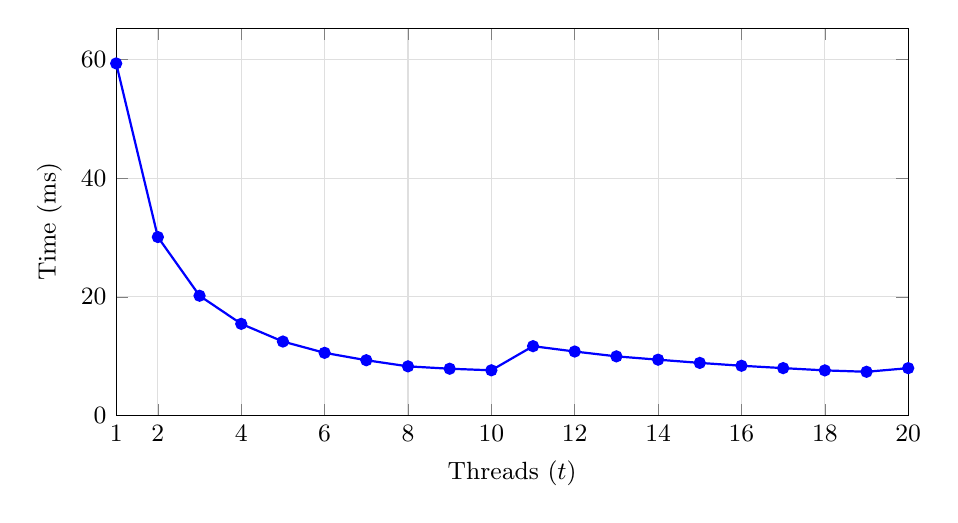
\begin{tikzpicture}
\begin{axis}[width=0.96\linewidth,height=6.5cm,
xlabel={Threads ($t$)},ylabel={Time (ms)},
xmin=1,xmax=20,xtick={1,2,4,6,8,10,12,14,16,18,20},
ymin=0,grid=both,major grid style={gray!25},minor grid style={gray!10},
tick label style={font=\small},label style={font=\small},
scaled y ticks=false,/pgf/number format/1000 sep={}]
\addplot[blue,thick,mark=*,mark size=1.8pt] coordinates {
(1, 59.356959)
(2, 30.08682)
(3, 20.188375)
(4, 15.450847)
(5, 12.469043)
(6, 10.566024)
(7, 9.318026)
(8, 8.285581)
(9, 7.883735)
(10, 7.620511)
(11, 11.687551)
(12, 10.785457)
(13, 9.968445)
(14, 9.409458)
(15, 8.86755)
(16, 8.384263)
(17, 7.988066)
(18, 7.605232)
(19, 7.368248)
(20, 7.981307)
};
\end{axis}
\end{tikzpicture}

{\small Matrix multiplication: $n=1024$.}
\end{center}
\newpage
\section*{Task 2}
An OpenMP parallel loop distributes output rows among threads. The input image and mask are read-only, and each output pixel has a private accumulator. The HW02 boundary convention is preserved: ones on edge strips and zeros where both coordinates are outside the image.

For $n=1024$ and a $3\times3$ mask, the time at one thread was 11.784 ms. The fastest median was 1.6188 ms at 10 threads ($7.279\times$ speedup). At 20 threads the time was 1.8323 ms, 13.187\% above the minimum; using all 20 threads did not improve the measured minimum. Increasing from 10 to 20 threads changed the time from 1.6188 to 1.8323 ms, so the additional threads did not reduce runtime in that comparison.

A plausible explanation for diminishing returns is that each pixel requires little work: OpenMP team and scheduling costs become substantial, while threads share caches and memory bandwidth. These are performance interpretations; the timing experiment does not measure those costs separately.
\begin{center}
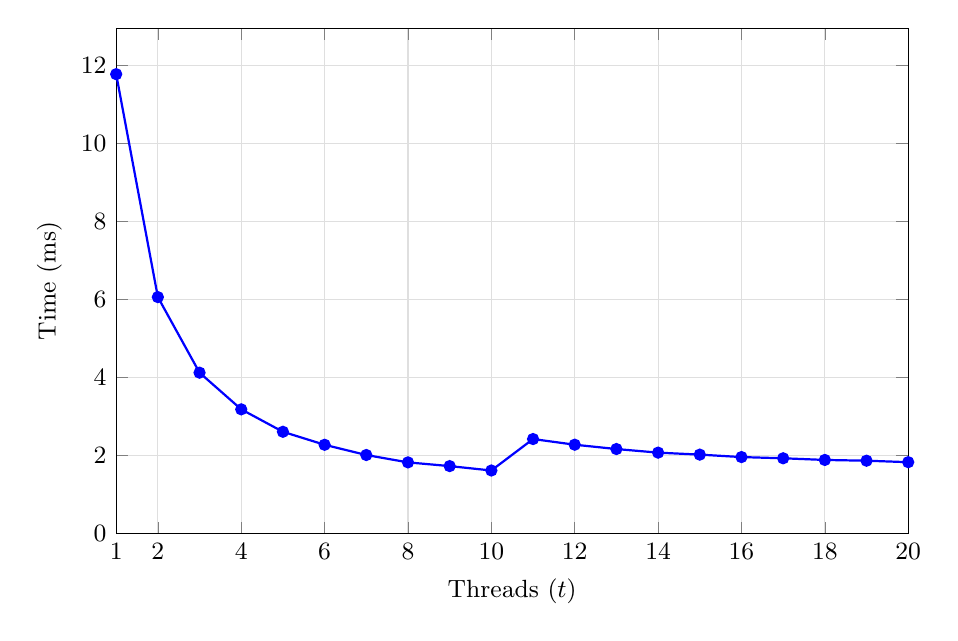
\begin{tikzpicture}
\begin{axis}[width=0.96\linewidth,height=8cm,
xlabel={Threads ($t$)},ylabel={Time (ms)},
xmin=1,xmax=20,xtick={1,2,4,6,8,10,12,14,16,18,20},
ymin=0,grid=both,major grid style={gray!25},minor grid style={gray!10},
tick label style={font=\small},label style={font=\small},
scaled y ticks=false,/pgf/number format/1000 sep={}]
\addplot[blue,thick,mark=*,mark size=1.8pt] coordinates {
(1, 11.783552)
(2, 6.065859)
(3, 4.12759)
(4, 3.187407)
(5, 2.611829)
(6, 2.278323)
(7, 2.01604)
(8, 1.827026)
(9, 1.731696)
(10, 1.618834)
(11, 2.425656)
(12, 2.280163)
(13, 2.169242)
(14, 2.07684)
(15, 2.025849)
(16, 1.963159)
(17, 1.932248)
(18, 1.889358)
(19, 1.869858)
(20, 1.832307)
};
\end{axis}
\end{tikzpicture}

{\small Convolution: $n=1024$, mask size $3\times3$.}
\end{center}
\newpage
\section*{Task 3}
Merge sort creates tasks for the two halves, waits for both, and then merges their sorted results. Below the threshold, iterative heap sorting avoids recursive calls and task creation.

For $n=10^6$ and eight threads, the best tested threshold was $ts=256$, with a median time of 15.926 ms. The smallest threshold, $ts=2$, took 1345.5 ms. Small thresholds create many tiny tasks, increasing scheduling overhead. Large thresholds leave more work in serial leaf sorts; the sweep measures this tradeoff for the tested implementation and node.
\begin{center}
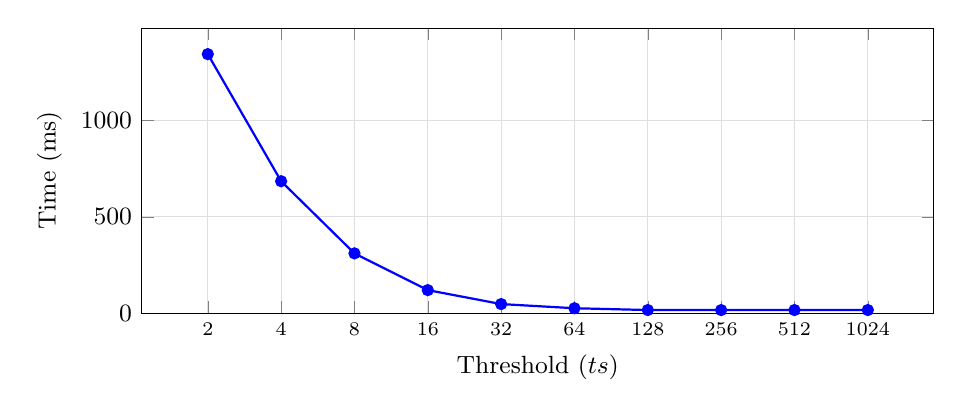
\begin{tikzpicture}
\begin{axis}[width=0.96\linewidth,height=5.2cm,
xlabel={Threshold ($ts$)},ylabel={Time (ms)},
xmode=log,log basis x=2,xtick={2,4,8,16,32,64,128,256,512,1024},xticklabels={2,4,8,16,32,64,128,256,512,1024},x tick label style={font=\scriptsize},
ymin=0,grid=both,major grid style={gray!25},minor grid style={gray!10},
tick label style={font=\small},label style={font=\small},
scaled y ticks=false,/pgf/number format/1000 sep={}]
\addplot[blue,thick,mark=*,mark size=1.8pt] coordinates {
(2, 1345.547635)
(4, 685.272607)
(8, 310.478245)
(16, 119.603401)
(32, 47.15816)
(64, 25.506483)
(128, 16.135097)
(256, 15.926473)
(512, 16.072596)
(1024, 16.124346)
};
\end{axis}
\end{tikzpicture}

{\small Threshold sweep: $n=10^6$, $t=8$; logarithmic horizontal axis.}
\end{center}
At $ts=256$, the fastest thread count was 19 (11.963 ms). One thread took 56.923 ms and 20 threads took 12.149 ms ($4.6854\times$ speedup). Serial merging near the top of the recursion tree and task overhead limit ideal scaling.
\begin{center}
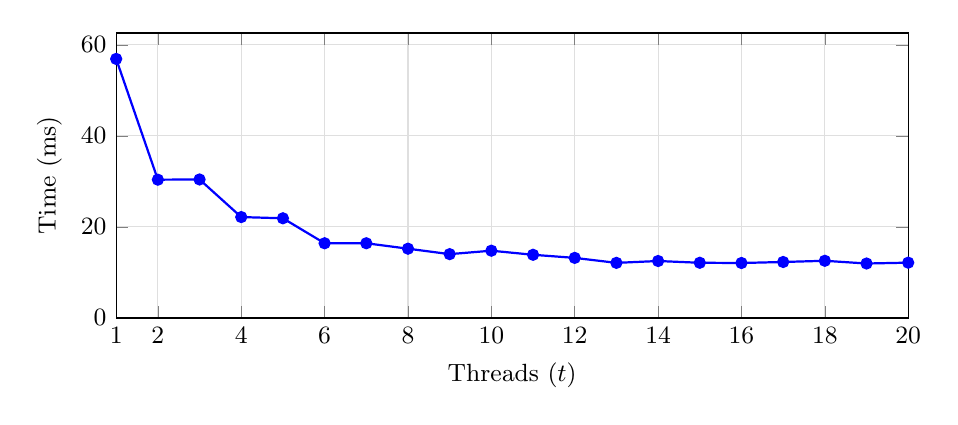
\begin{tikzpicture}
\begin{axis}[width=0.96\linewidth,height=5.2cm,
xlabel={Threads ($t$)},ylabel={Time (ms)},
xmin=1,xmax=20,xtick={1,2,4,6,8,10,12,14,16,18,20},
ymin=0,grid=both,major grid style={gray!25},minor grid style={gray!10},
tick label style={font=\small},label style={font=\small},
scaled y ticks=false,/pgf/number format/1000 sep={}]
\addplot[blue,thick,mark=*,mark size=1.8pt] coordinates {
(1, 56.923203)
(2, 30.385435)
(3, 30.432386)
(4, 22.169894)
(5, 21.902259)
(6, 16.41253)
(7, 16.414411)
(8, 15.218563)
(9, 14.021936)
(10, 14.779086)
(11, 13.881864)
(12, 13.198704)
(13, 12.105628)
(14, 12.511484)
(15, 12.125598)
(16, 12.075057)
(17, 12.297321)
(18, 12.560284)
(19, 11.962966)
(20, 12.149067)
};
\end{axis}
\end{tikzpicture}

{\small Thread sweep: $n=10^6$, selected threshold $ts=256$.}
\end{center}
\end{document}
